\documentclass[11pt,a4paper]{article}

\usepackage{acet}
\usepackage{times}
\usepackage{latexsym}
\usepackage{url}
\usepackage{color,graphicx} % for dvips(k)
\usepackage{amsmath,amssymb,amsfonts}
\usepackage{algorithmic}
\usepackage{array}
\usepackage{fancyhdr}

\title{Building a Khmer Traffic Sign Dataset for Automated Detection and Classification}
\author{Sophearith Chren\and Second Author\and Third Author\and Fourth Author\\
\small Department of Computer Science of Cambodia Academy of Digital Technology,\\
\small Phnom Penh Cambodia \\
{\tt corresponding\_author@cadt.edu.kh}}

\summary{
Traffic Sign Detection and Classification have become a core feature of computer vision, contributing
for intelligent transportation systems, traffic monitoring and driver assistance technologies. However,
the availability of public datasets illustrating Khmer traffic signs remains limited, making it challenging
to develop and evaluate reliable detection and classification models for Cambodia. To overcome the lack of the publicly available 
Khmer datasets, this research introduces a custom Khmer traffic sign datasets collected and annotated 
the capture image from various locations in Cambodia. The datasets contain an image captured under multiple 
real-world conditions including differnt lighting, different angles, distance, background and covers 42 classes commonly found in Cambodia. 
To evaluate the dataset, YOLOv8 and YOLOv10 models were trained and compared.
YOLOv8 achieved the best performance with an accuracy of 93\%
on the primary dataset and was integrated into a bilingual web-based application supporting both Khmer and English languages for automated traffic sign detection and classification.
This system demonstrates the practical application of deep learning-based Khmer traffic sign
recognition and provides a foundation for future research and intelligent transportation applications in Cambodia.
}
\begin{document}
\maketitle

\medskip
\noindent{\bf\textit{Keywords:}} \textit{Khmer Traffic Sign, Khmer Traffic Sign Detection and Classification (KTSDC), Computer Vision, Deep Learning}

\section{Introduction}

Traffic Signs play a significance role in modern transportation systems by providing an importance information, guiding driver behavior and enhancing road safety \cite{ertler-2020}\cite{farag-2019}. 
With the rapid of development of computer vision and deep learning techniques, automated traffic sign detection and classification have become main research areas for intelligent transportation systems and driver assistance technologies.

Developing accurate and reliable traffic sign detection and classification models require a large-scale dataset. Existing datasets, including German Traffic Sign Recognition Benchmark (GTSRB) \cite{stallkamp-2012},
Mapillary Traffic Sign Dataset (MTSD) \cite{ertler-2020}, Tsinghua-Tencent 100K (TT100K) \cite{zhu2016}, provide comprehensive coverage for their regions. However, they are limited for specific countries and do not effectively represent 
the traffic sign used in Cambodia \cite{ertler-2020}, \cite{stallkamp-2012}, \cite{zhu2016}. 

In Cambodia, the availability of publicly accessed Khmer traffic sign datasets remains limited \cite{ratitya2025}. Existing research on Cambodian traffic signs focuses only on seven classes \cite{ratitya2025}, which do not fully represent the wide range of
usually found in Cambodia roadways. Therefore, this limitation highlights a significant research gap in the development of a complete KTSDC system.

To address this research gap, this study proposes a KTSDC system based on a custom traffic sign dataset that was collected and annotated from various locations across Cambodia. 
The proposed collection consists of 42 classes of traffic sign types collected under various real-world conditions, including different lighting, different angles, distances, and backgrounds.
Furthermore, YOLOv8 and YOLOv10 were trained and evaluated to find out the effectiveness for Khmer traffic sign detection and classification.

\section{Dataset}
In this section, we will describe the custom Khmer traffic sign dataset produced in this project. 
The dataset was manually collected and annotated for traffic sign detection and classification in Cambodia road environments.
\subsection{Dataset Overview}
This paper introduces custom Khmer traffic sign dataset designed for traffic sign detection and classification in Cambodia road conditions.
The proposed dataset was collected and annotated by our team, which consisted of 42 classes that consisting several categories including
regulation, warning, required, and informational signals. The collected images demonstrate various real-world environments with differences
in lighting, angles, distances and backgrounds. Figure 1 demonstrates the complete set of traffic sign classes included in the proposed dataset.
In the next section will detail the data collection, annotation and data statistics.
\begin{figure}[ht]
\fontsize{18}{8}\selectfont 
\begin{center}
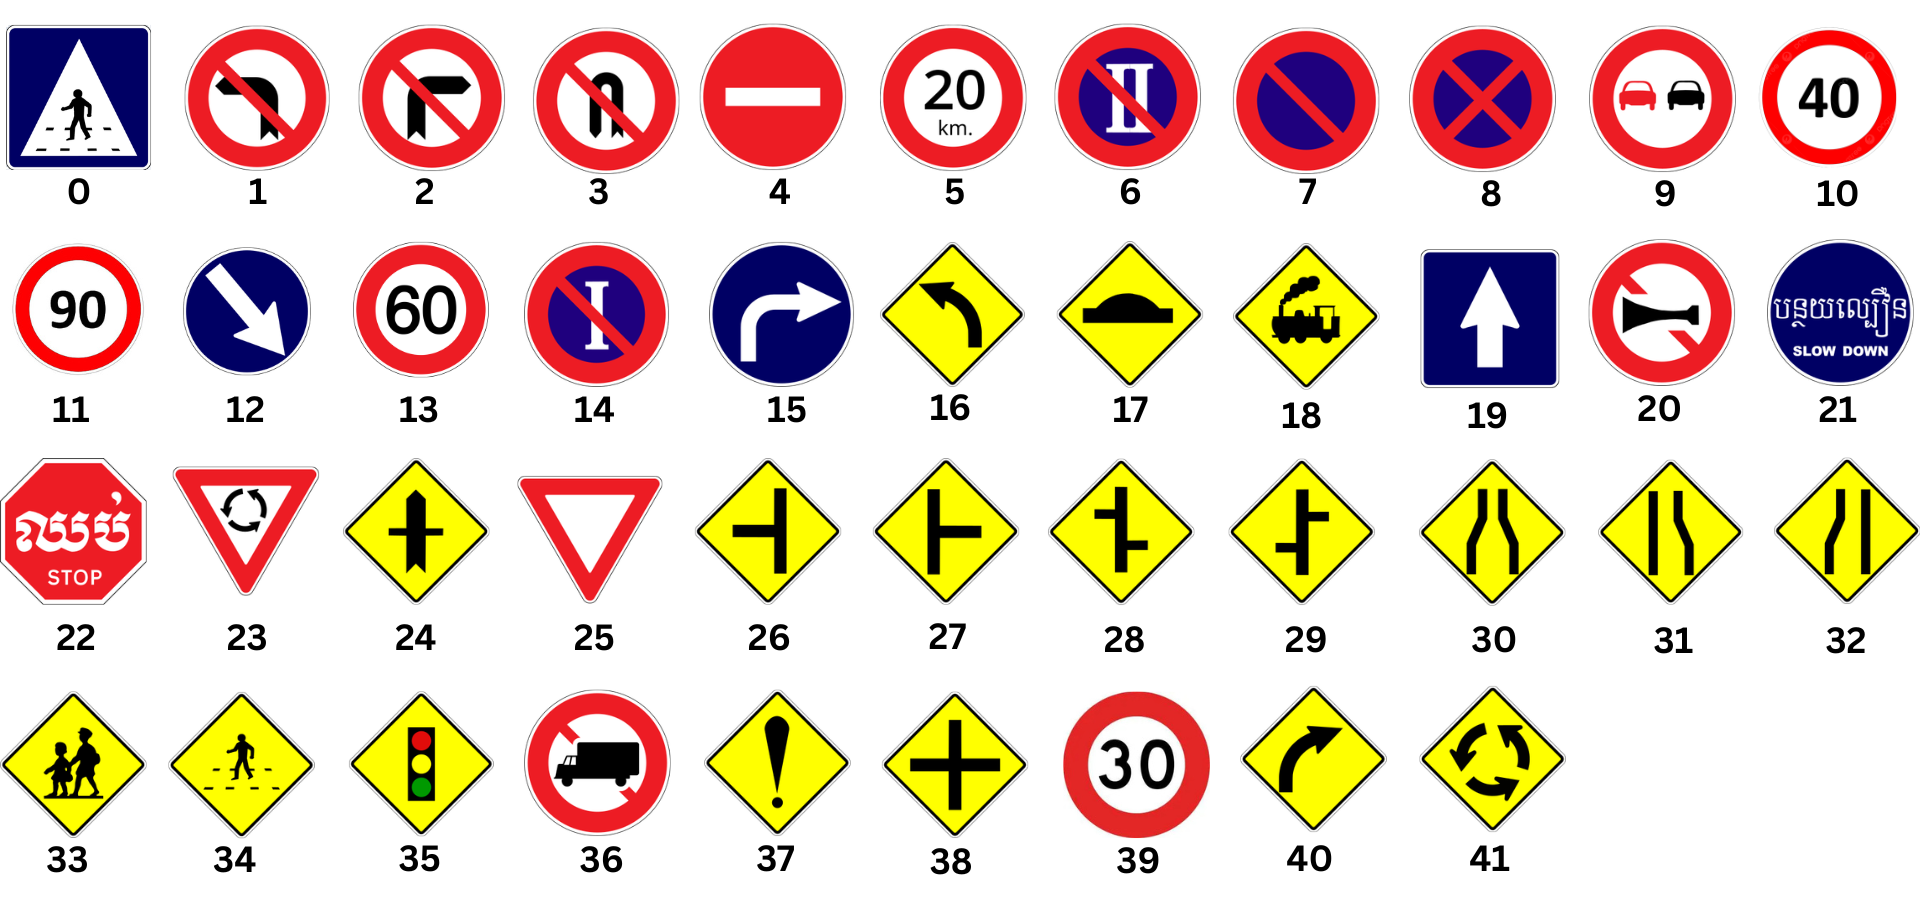
\includegraphics[width=7.4cm]{./fig/Sign_classes.png}
\caption{The 42 traffic sign classes included in the proposed dataset} 
\label{fig:sign_classes}
\end{center}
\end{figure} 
\subsection{Data Collection}
The traffic sign images were manually collected by our team from several sites across Cambodia using a smartphone camera.
Data collecting was conducted on a few different road types, which include urban streets and rural streets. Images were taken under different
real-world conditions, such as different lighting conditions, viewing angles, object distances, and background environments, to boost dataset diversity.
After data gathering, all the images were carefully reviewed to remove duplicate images, images without traffic signs, and images that contain poor visibility that
prevented clear identification of the traffic signs. This process ensured that only the quality images were left for data annotation process.
\subsection{Data Annotation}
Following data collection, all the images were manually annotated using the CVAT annotation tool. Each traffic sign was allocated a rectangular bounding box and
provided with a class label according to one of the 42 predefined traffic sign classes. The annotations were exported in the YOLO format, containing the class
identifier and normalized bounding box coordinates for each signs. To ensure annotations quality, all annotations have been manually validated by our team, and incorrect class labels or inaccurate
bounding boxes were fixed before finish datasets.
\begin{figure}[ht]
    \centering
    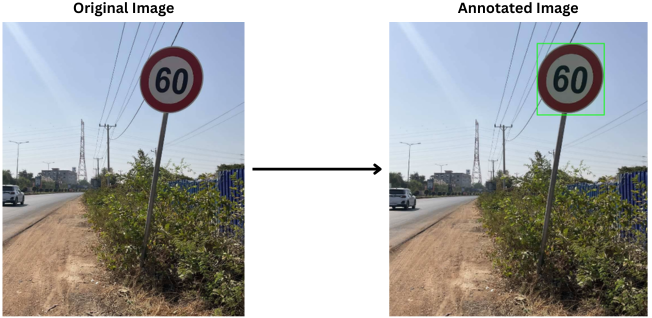
\includegraphics[width=7.4cm]{./fig/Annotated_Image.png}
    \caption{Example of the traffic sign annotation process. Original image. Annotated image with bounding box and class label generated using CVAT}
    \label{fig:annotation}
\end{figure}
\subsection{Data Statistics}
\section{Methodology}
The following section discusses the techniques utilized to develop and create the Khmer traffic sign detection and classification approach.
The overall research process and experimental procedures are describe in the following section.
\subsection{Methodology Workflow}
The proposed methodlogy establishes a systematic workflow for Khmer traffic sign detection and classification.
The process begins with data preparation and data preprocessing for the annotated traffic sign dataset, followed by the model development
and training under experimental set up. After training, the models will evaluated on the test dataset using standard object detection metrics.
The obtained results are subsequently compared to identify model that achieves performance for Khmer dataset. 
\subsection{Data Preprocessing}

\subsection{Model Development}
\subsection{Model Training}
\subsection{Evaluation}
\begin{table*}[ht]
\caption{Units for Magnetic Properties}
\label{fontstyle}
\centering
\begin{tabular}{lcccc} \hline\hline
Subset & Total & Training & Validation & Testing \\ \hline
Images &
31667&
22148 \\
Labels &
31544&
22064\\
Bouding Box &
32036&
22400 \\
\hline\hline
\end{tabular}
\end{table*}

\subsection{Title, authors' names and affiliations}

Place the title at the top of the first page, followed by the authors' names and their affiliations.  Long title should be typed on two lines without a blank line intervening.  The title of the paper should be written in bold in 14 point font.  The first letter of word except preposition (i.e., of, with, on, in, for), definite article (the) and indefinite article (a, an) in the title should be capitalized. The authors name' must be in bold in 12 point font, followed the title with a line space skipped.  The affiliation should followed the authors name,
in 12 point font.

Center the title across both columns.  Use the two-column format only when you begin the abstract.  Note for \LaTeX{}, use \verb+\and+ to separate authors from the same affiliation, and \verb+\AND+ for starting an author block in the separated line.

\subsection{Text}

Begin typing the main body of the text immediately after the keywords with 11 point font, observing the two-column format as shown in this example.

Type and label section headings in 12pt bold font.  Use numbered
sections, in order to facilitate cross references.

Type and label section headings in 11pt bold font.  Use numbered
sections, in order to facilitate cross references.

\subsection{Equations}
Number equations consecutively with equation numbers in parentheses flush with the right margin, as in \eqref{eq}. To make your equations more compact, you may use the solidus (~/~), the exp function, or appropriate exponents. Use parentheses to avoid ambiguities in denominators. Punctuate equations when they are part of a sentence, as in
\begin{equation}E=mc^2.\label{eq}\end{equation}

The following equation are used to test your LaTeX compiler's math output. Equation (2) is your LaTeX compiler' output. 

\begin{align*} \frac{4i+8jk\times 10rym }{(6\pi) Aoq \sum _{i=1}^{r} Q(t)} {\int\limits_0^\infty \! f(g)\mathrm{d}x}  \sqrt[3]{\frac{abcdelqh^2}{ (svw) \cos^3\theta }} . \tag{2}\end{align*}

Be sure that the symbols in your equation have been defined before the equation appears or immediately following. Italicize symbols ($T$ might refer to temperature, but T is the unit tesla). Refer to ``\eqref{eq},'' not ``Eq. \eqref{eq}''
or ``equation \eqref{eq},'' except at the beginning of a sentence: ``Equation \eqref{eq}
is $\ldots$ .''

\subsection{Graphics}
Format and save your graphics using a suitable graphics processing program that will allow you to create the images as PostScript (.PS), Encapsulated PostScript (.EPS), Tagged Image File Format (.TIFF), Portable Document Format (.PDF), Portable Network Graphics (.PNG), or Metapost (.MPS), sizes them, and adjusts the resolution settings. When submitting your final paper, your graphics should all be submitted individually in one of these formats along with the manuscript.

{\bf Illustrations}: Place figures, tables, and photographs in the paper near where they are first discussed, rather than at the end, if possible.  Wide illustrations may run across both columns.  See \figref{sampleimg} for include an illustration.

\begin{figure}[ht]
\fontsize{18}{8}\selectfont 
\begin{center}

\includegraphics[width=7cm]{./fig/ACET_logo.png}
\caption{Sample Image} 
\label{sampleimg}
\end{center}
\end{figure} 

{\bf Captions}: Provide a caption for every illustration; number each one sequentially in the form: ``Figure 1:  Caption of the Figure.'' ``Table 1:  Caption of the Table.''  Type the captions for figures below the figures.  Type the captions for tables above the tables (see \figref{fontstyle}).

\subsection{Appendices and References}
{\bf Appendixes}: Appendixes, if any, directly follow the text and the references (but see above).  Letter them in sequence and provide an informative title: {\bf Appendix A. Title of Appendix.}

{\bf References}: Citations within the text appear in bracket as
[Number] such as \cite{ACM:83}, \cite{APA}, \cite{Vichet_2015}, \cite{Ye_KhmerSMT_2015} and \cite{Ye_KhmerPOS_2017}.  Gather the full set of references together under the heading {\bf References}; place the section before any {\bf Appendices}, unless they contain references. Provide as complete a citation as possible, using a consistent format.

\textbf{BibTeX} does not work by magic. It doesn't get the bibliographic data from thin air but from .bib files. If you use \textbf{BibTeX} to produce a bibliography you must send the .bib files.

ACET follows the IEEE's reference style, which the preparation guideline can be found below:\\
•	Basic format for books:
J. K. Author, “Title of chapter in the book,” in Title of His Published Book, xth ed. City of Publisher, (only U.S. State), Country: Abbrev. of Publisher, year, ch. x, sec. x, pp. xxx–xxx.\\
See [1], [2]. \\
•	Basic format for periodicals:
J. K. Author, “Name of paper,” Abbrev. Title of Periodical, vol. x, no. x, pp. xxx–xxx, Abbrev. Month, year, DOI. 10.1109.XXX.123456.\\
See [3]–[5]. \\
•	Basic format for reports:
J. K. Author, “Title of report,” Abbrev. Name of Co., City of Co., Abbrev. State, Country, Rep. xxx, year.\\
See [6], [7]. \\
•	Basic format for handbooks:
Name of Manual/Handbook, x ed., Abbrev. Name of Co., City of Co., Abbrev. State, Country, year, pp. xxx–xxx.\\
See [8], [9]. \\
•	Basic format for books (when available online):
J. K. Author, “Title of chapter in the book,” in Title of Published Book, xth ed. City of Publisher, State,  Country: Abbrev. of Publisher, year, ch. x, sec. x, pp. xxx–xxx. [Online]. Available: http://www.web.com\\
See [10]–[13]. \\
•	Basic format for journals (when available online):
J. K. Author, “Name of paper,” Abbrev. Title of Periodical, vol. x, no. x, pp. xxx–xxx, Abbrev. Month, year. Accessed on: Month, Day, year, DOI: 10.1109.XXX.123456, [Online].\\
See [14]–[16]. \\
•	Basic format for papers presented at conferences (when available online):
J.K. Author. (year, month). Title. presented at abbrev. conference title. [Type of Medium]. Available: site/path/file\\
See [17]. \\
•	Basic format for reports and handbooks (when available online):
J. K. Author. “Title of report,” Company. City, State, Country. Rep. no., (optional: vol./issue), Date. [Online] Available: site/path/file\\
See [18], [19]. \\
•	Basic format for computer programs and electronic documents (when available online):
Legislative body. Number of Congress, Session. (year, month day). Number of bill or resolution, Title. [Type of medium]. Available: site/path/file\\
See [20]. \\
•	Basic format for patents (when available online): 
Name of the invention, by inventor’s name. (year, month day). Patent Number [Type of medium]. Available: site/path/file\\
See [21]. \\
•	Basic format for conference proceedings (published):
J. K. Author, “Title of paper,” in Abbreviated Name of Conf., City of Conf., Abbrev. State (if given), Country, year, pp. xxxxxx.\\
See [22]. \\
•	Example for papers presented at conferences (unpublished):
See [23].\\
•	Basic format for patents:
J. K. Author, “Title of patent,” U.S. Patent x xxx xxx, Abbrev. Month, day, year.\\
See [24]. \\
•	Basic format for theses (M.S.) and dissertations (Ph.D.):
1)	J. K. Author, “Title of thesis,” M.S. thesis, Abbrev. Dept., Abbrev. Univ., City of Univ., Abbrev. State, year.
2)	J. K. Author, “Title of dissertation,” Ph.D. dissertation, Abbrev. Dept., Abbrev. Univ., City of Univ., Abbrev. State, year.\\
See [25], [26]. \\
•	Basic format for the most common types of unpublished references:\\
1)	J. K. Author, private communication, Abbrev. Month, year.\\
2)	J. K. Author, “Title of paper,” unpublished.\\
3)	J. K. Author, “Title of paper,” to be published.\\
See [27]–[29]. \\
•	Basic formats for standards:\\
1)	Title of Standard, Standard number, date.\\
2)	Title of Standard, Standard number, Corporate author, location, date.\\
See [30], [31]. \\
•	Article number in reference examples:
See [32], [33].\\
•	Example when using et al.:
See [34].

\section{Style of Camera-Ready Manuscript}

The maximum length of camera-ready manuscripts is limited up to eight (9) pages of content, plus unlimited pages of references. All illustrations, references, and appendices must be accommodated within these page limits, also observing the formatting instructions given in the present document.  {\bf Note that DO NOT put a page number in each page.}

\section{Conclusion}
Although a conclusion may review the  main points of the paper, do not replicate the abstract as the conclusion. A
conclusion might elaborate on the importance of the work or suggest applications and extensions.


\subsection*{Acknowledgment}

Thanks to XXXXXXXXXXX.  This format is a modification of ONA 2018, SNLP 2013, KICSS2006 and IJCKS2007 style file.


% fdkjfdkfd \cite{chakraborty2014compact} kfkdfd.

% \bibliographystyle{unsrt}
% \bibliography{acet-sample}

\bibliographystyle{IEEEtran}
\bibliography{references/references}

% \begin{thebibliography}{00}

% \bibitem{b1} G. O. Young, ``Synthetic structure of industrial plastics,'' in \emph{Plastics,} 2\textsuperscript{nd} ed., vol. 3, J. Peters, Ed. New York, NY, USA: McGraw-Hill, 1964, pp. 15--64.

% \bibitem{b2} W.-K. Chen, \emph{Linear Networks and Systems.} Belmont, CA, USA: Wadsworth, 1993, pp. 123--135.

% \bibitem{b3} J. U. Duncombe, ``Infrared navigation---Part I: An assessment of feasibility,'' \emph{IEEE Trans. Electron Devices}, vol. ED-11, no. 1, pp. 34--39, Jan. 1959, 10.1109/TED.2016.2628402.

% \bibitem{b4} E. P. Wigner, ``Theory of traveling-wave optical laser,'' \emph{Phys. Rev}., vol. 134, pp. A635--A646, Dec. 1965.

% \bibitem{b5} E. H. Miller, ``A note on reflector arrays,'' \emph{IEEE Trans. Antennas Propagat}., to be published.

% \bibitem{b6} E. E. Reber, R. L. Michell, and C. J. Carter, ``Oxygen absorption in the earth's atmosphere,'' Aerospace Corp., Los Angeles, CA, USA, Tech. Rep. TR-0200 (4230-46)-3, Nov. 1988.

% \bibitem{b7} J. H. Davis and J. R. Cogdell, ``Calibration program for the 16-foot antenna,'' Elect. Eng. Res. Lab., Univ. Texas, Austin, TX, USA, Tech. Memo. NGL-006-69-3, Nov. 15, 1987.

% \bibitem{b8} \emph{Transmission Systems for Communications}, 3\textsuperscript{rd} ed., Western Electric Co., Winston-Salem, NC, USA, 1985, pp. 44--60.

% \bibitem{b9} \emph{Motorola Semiconductor Data Manual}, Motorola Semiconductor Products Inc., Phoenix, AZ, USA, 1989.

% \bibitem{b10} G. O. Young, ``Synthetic structure of industrial
% plastics,'' in Plastics, vol. 3, Polymers of Hexadromicon, J. Peters,
% Ed., 2\textsuperscript{nd} ed. New York, NY, USA: McGraw-Hill, 1964, pp. 15-64.
% [Online]. Available:
% \underline{http://www.bookref.com}.

% \bibitem{b11} \emph{The Founders' Constitution}, Philip B. Kurland
% and Ralph Lerner, eds., Chicago, IL, USA: Univ. Chicago Press, 1987.
% [Online]. Available: \underline{http://press-pubs.uchicago.edu/founders/}

% \bibitem{b12} The Terahertz Wave eBook. ZOmega Terahertz Corp., 2014.
% [Online].Available:\underline{http://dl.zthz.com.pdf}. Accessed on: May 19, 2014.

% \bibitem{b13} Philip B. Kurland and Ralph Lerner, eds., \emph{The
% Founders' Constitution.} Chicago, IL, USA: Univ. of Chicago Press,
% 1987, Accessed on: Feb. 28, 2010, [Online] Available:
% \underline{http://press-pubs.uchicago.edu/founders/}

% \bibitem{b14} J. S. Turner, ``New directions in communications,'' \emph{IEEE J. Sel. Areas Commun}., vol. 13, no. 1, pp. 11-23, Jan. 1995.

% \bibitem{b15} W. P. Risk, G. S. Kino, and H. J. Shaw, ``Fiber-optic frequency shifter using a surface acoustic wave incident at an oblique angle,'' \emph{Opt. Lett.}, vol. 11, no. 2, pp. 115--117, Feb. 1986.

% \bibitem{b16} P. Kopyt \emph{et al., ``}Electric properties of graphene-based conductive layers from DC up to terahertz range,'' \emph{IEEE THz Sci. Technol.,} to be published. DOI: 10.1109/TTHZ.2016.2544142.

% \bibitem{b17} PROCESS Corporation, Boston, MA, USA. Intranets:
% Internet technologies deployed behind the firewall for corporate
% productivity. Presented at INET96 Annual Meeting. [Online].
% Available: \underline{http://home.process.com/Intranets/wp2.htp}

% \bibitem{b18} R. J. Hijmans and J. van Etten, ``Raster: Geographic analysis and modeling with raster data,'' R Package Version 2.0-12, Jan. 12, 2012. [Online]. Available: \underline {http://CRAN.R-project.org/package=raster}

% \bibitem{b19} Teralyzer. Lytera UG, Kirchhain, Germany [Online].
% Available:\underline{http://www.lytera.de}, Accessed on: Jun. 5, 2014.

% \bibitem{b20} U.S. House. 102\textsuperscript{nd} Congress, 1\textsuperscript{st} Session. (1991, Jan. 11). \emph{H. Con. Res. 1, Sense of the Congress on Approval of}  \emph{Military Action}. [Online]. Available: LEXIS Library: GENFED File: BILLS

% \bibitem{b21} Musical toothbrush with mirror, by L.M.R. Brooks. (1992, May 19). Patent D 326 189 [Online]. Available: NEXIS Library: LEXPAT File: DES

% \bibitem{b22} D. B. Payne and J. R. Stern, ``Wavelength-switched pas- sively coupled single-mode optical network,'' in \emph{Proc. IOOC-ECOC,} Boston, MA, USA, 1985, pp. 585--590.

% \bibitem{b23} D. Ebehard and E. Voges, ``Digital single sideband detection for interferometric sensors,'' presented at the \emph{2\textsuperscript{nd} Int. Conf. Optical Fiber Sensors,} Stuttgart, Germany, Jan. 2-5, 1984.

% \bibitem{b24} G. Brandli and M. Dick, ``Alternating current fed power supply,'' U.S. Patent 4 084 217, Nov. 4, 1978.

% \bibitem{b25} J. O. Williams, ``Narrow-band analyzer,'' Ph.D. dissertation, Dept. Elect. Eng., Harvard Univ., Cambridge, MA, USA, 1993.

% \bibitem{b26} N. Kawasaki, ``Parametric study of thermal and chemical nonequilibrium nozzle flow,'' M.S. thesis, Dept. Electron. Eng., Osaka Univ., Osaka, Japan, 1993.

% \bibitem{b27} A. Harrison, private communication, May 1995.

% \bibitem{b28} B. Smith, ``An approach to graphs of linear forms,'' unpublished.

% \bibitem{b29} A. Brahms, ``Representation error for real numbers in binary computer arithmetic,'' IEEE Computer Group Repository, Paper R-67-85.

% \bibitem{b30} IEEE Criteria for Class IE Electric Systems, IEEE Standard 308, 1969.

% \bibitem{b31} Letter Symbols for Quantities, ANSI Standard Y10.5-1968.

% \bibitem{b32} R. Fardel, M. Nagel, F. Nuesch, T. Lippert, and A. Wokaun, ``Fabrication of organic light emitting diode pixels by laser-assisted forward transfer,'' \emph{Appl. Phys. Lett.}, vol. 91, no. 6, Aug. 2007, Art. no. 061103.~

% \bibitem{b33} J. Zhang and N. Tansu, ``Optical gain and laser characteristics of InGaN quantum wells on ternary InGaN substrates,'' \emph{IEEE Photon. J.}, vol. 5, no. 2, Apr. 2013, Art. no. 2600111

% \bibitem{b34} S. Azodolmolky~\emph{et al.}, Experimental demonstration of an impairment aware network planning and operation tool for transparent/translucent optical networks,''~\emph{J. Lightw. Technol.}, vol. 29, no. 4, pp. 439--448, Sep. 2011.

% \end{thebibliography}

\end{document}
